% Giacomo Petrillo
% lezione di Punzi

% parte sulle sistematiche spostata dalla lezione 10 ottobre
\section{Sistematiche}

Quando non siamo sicuri sul modello da usare,
diciamo che abbiamo un'\emph{incertezza sistematica}.
Per trattare statisticamente l'incertezza sistematica,
bisogna fissare una famiglia di modelli.
L'unione di una famiglia di modelli è ancora un modello,
quindi a questo punto si può:
\begin{itemize}
	\item fare inferenza sul modello complessivo;
	\item fare una famiglia di inferenze.
\end{itemize}

\begin{example}
	Consideriamo un modello gaussiano di variabili $y_i$
	con media $\mu_i(\theta)$ funzione del parametro e varianze $\sigma_i^2$:
	\begin{equation*}
		p(\mathbf y;\theta)
		= \prod_i \frac1{\sqrt{2\pi}\sigma_i}
		\exp\left(-\frac12\left(\frac{y_i-\mu_i(\theta)}{\sigma_i}\right)^2\right).
	\end{equation*}
	Supponiamo di avere un dubbio su quali siano le $\sigma_i$.
	In generale il valore delle $\sigma_i$ influenzerà il risultato per $\theta$.
	Allora possiamo considerare le $\sigma_i$ come un parametro
	e fare inferenza sia su $\theta$ che sulle varianze:
	\begin{equation*}
		p(\mathbf y;\theta) \rightarrow p(\mathbf y;\theta,\boldsymbol\sigma).
	\end{equation*}
	Un modo più ``agnostico'' di risolvere la questione è tenere le $\sigma_i$ fissate
	e dire quale risultato si ottiene per $\theta$ al variare delle $\sigma_i$
	tra alcuni valori di interesse.
\end{example}

\begin{figure}
	\centering
	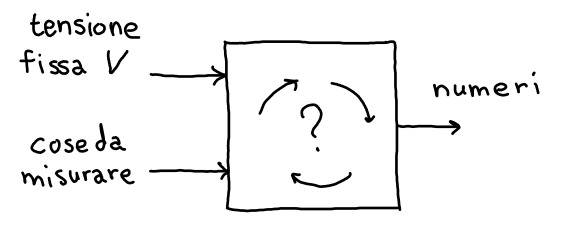
\includegraphics[width=20em]{macchinario}
	\caption{\label{fig:macchinario}
	Esempio generico di un apparato di misura il cui risultato,
	oltre che dalle cose che vogliamo misurare,
	dipende da altre condizioni che quindi vanno altresì misurate.
	Ad esempio un macchinario la cui calibrazione dipende dalla tensione di alimentazione.}
\end{figure}

\begin{example}
	Consideriamo un esperimento in cui abbiamo un macchinario dal funzionamento complicato
	da cui otteniamo dei numeri (i nostri dati),
	e in cui per ricavare il risultato che ci interessa dai dati
	dobbiamo anche misurare il potenziale elettrico di un certo punto del macchinario
	(vedi \autoref{fig:macchinario}).
	Ad esempio potrebbe essere un oscilloscopio la cui calibrazione dipende dalla tensione di alimentazione.
	Supponiamo di misurare questa tensione con un multimetro.
	Per trattare statisticamente l'incertezza della misura del multimetro,
	combiniamo il modello del macchinario con una gaussiana
	che ha per deviazione standard l'incertezza del multimetro:
	\begin{align*}
		\mathcal L
		&= P_\text{macchinario}(\text{dati}|\text{parametri, tensione}) \cdot \\
		&\cdot P_\text{multimetro}(\text{tensione misurata}|\text{tensione}), \\
		P_\text{multimetro}(V_\text{mis}|V)
		&= \frac 1 {\sqrt{2\pi}\sigma_\text{multimetro}}
		\exp \left( -\frac12 \left( \frac{V_\text{mis} - V} {\sigma_\text{multimetro}} \right)^2 \right).
	\end{align*}
	Quindi, se facciamo un fit, oltre ai parametri che ci interessano
	otterremo anche un risultato per la tensione
	(in generale i parametri che non ci interessano vengono chiamati \emph{nuisance parameters},
	letteralmente parametri fastidiosi).
	Supponiamo che, facendo un fit con il modello,
	il risultato per la tensione venga diverso di molte sigma rispetto a quello misurato.
	Poiché la misura della tensione è molto semplice,
	supponiamo che sia corretta,
	e riteniamo invece che il modello del macchinario abbia dei problemi, es. troppe approssimazioni.
	Allora facciamo il fit fissando la tensione a quella misurata:
	\begin{equation*}
		\mathcal L = P_\text{macchinario}(\text{dati}|\text{parametri, tensione misurata}),
	\end{equation*}
	e ripetiamo il fit variando la tensione che mettiamo di $\pm 1\sigma_\text{multimetro}$.
	La corrispondente variazione che otteniamo nel risultato la aggiungiamo in quadratura all'errore
	statistico del fit e diciamo che è una componente sistematica dell'incertezza.
	Questa procedura non è ben fondata statisticamente ma ci permette di riportare un risultato
	abbastanza sensato quando non sappiamo come procedere altrimenti.
\end{example}

Nota: spesso nei \emph{counting experiments},
cioè quelli in cui si contano degli eventi supposti poissoniani,
si intende con incertezza statistica la componente dell'incertezza dovuta alla varianza della poissoniana
e con incertezza sistematica tutto il resto,
anche se i nuisance parameters sono stati trattati statisticamente.
Questo perché tipicamente l'incertezza statistica scenderà come $1/\sqrt T$
dove $T$ è il tempo per cui lascio acceso l'esperimento,
mentre l'incertezza sistematica cambierà poco con la durata,
e questo è utile per sapere quanto tempo vale la pena continuare a prendere dati.

\section{Likelihood gaussiana}

Consideriamo la gaussiana con media $\mu$ e deviazione standard $\sigma$:
\begin{equation*}
	g(x;\mu,\sigma) \is \frac1{\sqrt{2\pi}\sigma} e^{-\frac12 \left( \frac{x-\mu}\sigma \right)^2}.
\end{equation*}
Calcoliamo la likelihood per $\mu$ con due misure:
\begin{align*}
	\mathcal L(\mu)
	&= g(x_1;\mu,\sigma) g(x_2;\mu,\sigma) = \\
	&= \frac1{2\pi\sigma^2}
	e^{\left( \frac{x_1-x_2}{2\sigma} \right)^2}
	e^{-\frac2{2\sigma^2} \left( \frac{x_1+x_2}2 - \mu \right)^2} = \\
	&= f(x_1,x_2) g \big( \mu;\bar x,\sigma/\sqrt2 \big).
\end{align*}
Dunque la likelihood per $\mu$ è gaussiana.
Notiamo che la distribuzione di $\bar x$ ha la stessa forma $g \big( \bar x;\mu,\sigma/\sqrt2 \big)$
e che questo non vale in generale, si pensi ad esempio alla distribuzione uniforme
in cui la somma di due variabili è triangolare mentre la likelihood per la media della distribuzione è un'iperbole troncata.

\section{Sufficienza}

\begin{definition}[Sufficienza]
	\label{th:suff}
	Consideriamo un modello per $x$ con parametro $\theta$ e una statistica $s$.
	Si dice che $s$ è \emph{sufficiente} per $\theta$ se la distribuzione di $x$ si fattorizza come
	$p(x;\theta) = f(x) p(s(x);\theta)$ con $f\ge0$.
\end{definition}

Il senso della definizione di sufficienza
è che la likelihood calcolata con una statistica sufficiente
è equivalente a quella calcolata direttamente con la variabile,
cioè cambia di una costante moltiplicativa positiva:
\begin{align*}
	\mathcal L_{x_0}(\theta)
	&= p(x_0;\theta) = f(x_0) p(s(x_0);\theta) \propto \\
	\propto \mathcal L_{s(x_0)}(\theta)
	&= p(s(x_0);\theta),
\end{align*}
quindi per scrivere la likelihood è sufficiente conoscere $s_0 \is s(x_0)$.

\begin{theorem}
	Se $s(x)$ è sufficiente per $\theta$,
	la probabilità condizionata $p(x|s)$ non dipende da $\theta$.
\end{theorem}

\begin{proof}
	Basta calcolarla:
	\begin{align*}
		p(x|s_0;\theta)
		&= \frac {p(x,s_0;\theta)} {p(s_0;\theta)} = \\
		&= \frac {p(x;\theta) \delta(s_0-s(x))} {p(s_0;\theta)} = \\
		&= \frac {f(x) p(s(x);\theta) \delta(s_0-s(x))} {p(s_0;\theta)} = \\
		&= f(x) \delta(s_0-s(x)) = \\
		&= f(x) \sum_{x'\in s^{-1}(s_0)} \frac {\delta(x-x')} {|s'(x')|}. \qedhere
	\end{align*}
\end{proof}

\begin{definition}
	Una statistica sufficiente $s$ è \emph{minimale} se
	\begin{equation*}
		\forall \sigma \text{ statistica sufficiente}\ \exists f\ \forall x:
		s(x) = f(\sigma(x)).
	\end{equation*}
\end{definition}
\noindent Nota: non è detto che la statistica sufficiente minimale sia unica.

\begin{theorem}
	\label{th:suffatt}
	Se, per una qualche funzione $g$, la probabilità di $x$ si fattorizza come
	\begin{equation*}
		p(x;\theta) = f(x)\cdot g(s(x),\theta)
	\end{equation*}
	con $f\ge 0$, allora $s$ è sufficiente.
\end{theorem}

\begin{proof}
	Calcoliamo la probabilità di $s(x)$:
	\begin{align*}
		p(s(x);\theta)
		&= \sum_{x':s(x')=s(x)} \frac{p(x';\theta)}{J(x')} = \\
		&= \sum_{x':s(x')=s(x)} \frac{f(x') g(s(x'),\theta)}{J(x')} = \\
		&= \left( \sum_{x':s(x')=s(x)} \frac{f(x')}{J(x')} \right) g(s(x),\theta),
	\end{align*}
	dove $J$ è il jacobiano di $s$.
	Se la somma su $x'$ è nulla,
	essendo $f\ge 0$ devono essere nulli tutti i termini quindi in particolare $f(x)$.
	Allora posso scrivere
	\begin{align*}
		p(x;\theta)
		&= F(x) p(s(x);\theta) \\
		\intertext{dove}
		F(x)
		&= \begin{cases}
			\displaystyle\frac{f(x)}{\sum_{x':s(x')=s(x)} \frac{f(x')}{J(x')}}
			& \text{se }\sum_{x':s(x')=s(x)} \frac{f(x')}{J(x')} \neq 0 \\
			0 & \text{altrimenti.}
		\end{cases} \qedhere
	\end{align*}
\end{proof}

\begin{fact}[Teorema di Darmois]
	\label{th:darmois}
	Sia $x$ variabile reale e $\fundef[\mathbf s_N]{\R^N}{\R^d}$ statistica sufficiente per $\theta$ di $N$ estrazioni di $x$ per ogni $N$.
	Se il supporto di $p(x;\theta)$ non dipende da $\theta$, allora necessariamente
	\begin{equation*}
		p(x;\theta) =
		\exp \left( \sum_{k=1}^d \alpha_k(x)a_k(\theta) + \beta(x) + \gamma(\theta) \right)
	\end{equation*}
	e la statistica sufficiente è, a meno di una funzione biunivoca,
	\begin{equation}
		\label{eq:statdarmois}
		s_{N,k}(\mathbf x) = \sum_{i=1}^{N} \alpha_k(x_i);
	\end{equation}
	le pdf in questa forma si chiamano \emph{famiglia esponenziale}.
	Viceversa, se la pdf è della famiglia esponenziale, la statistica \eqref{eq:statdarmois} è sufficiente.
\end{fact}

\begin{exercise}
	Dimostrare la seconda freccia del teorema di Darmois.
\end{exercise}

\begin{solution}
	Calcoliamo la pdf delle estrazioni:
	\begin{align*}
		p(\mathbf x;\mu)
		&= \prod_{k=1}^N p(x_k;\mu) = \\
		&= \exp \left( \sum_{k=1}^N \sum_{i=1}^d \alpha_i(x_k)a_i(\mu)
		+ \sum_{k=1}^N \beta(x_k) + N\gamma(\mu) \right) = \\
		&= \exp \left( \sum_{k=1}^N \beta(x_k) \right)
		\cdot \exp \left( \sum_{i=1}^d a_i(\mu)s_i(\mathbf x) + N\gamma(\mu) \right) = \\
		&= f(\mathbf x) \cdot g(\mathbf s(\mathbf x);\mu), \quad f\ge0.
	\end{align*}
	Il \autoref{th:suffatt} conclude.
	Notiamo che la dimostrazione vale anche se $x$ non è una variabile reale.
\end{solution}
